\begin{figure}
\centering
  \begin{tabular}{c}
  \begin{subfigure}{0.45\textwidth}
 \tabl{c}{\scalebox{0.8}{\begin{tikzpicture}
      \begin{axis}[
	xlabel={timestep},
	ylabel={Cumulative regret},
       clip mode=individual,grid,grid style={gray!30},
  legend style={at={(0.5,-0.2)},anchor=north,legend columns=3} ]
      % UCB
\addplot table[x index=0,y index=1,col sep=tab,each nth point={10}] {results/Expt1/clUCBcomp_subsampled.txt};
\addplot table[x index=0,y index=1,col sep=tab,each nth point={10}] {results/Expt1/DMEDcomp_subsampled.txt};
\addplot table[x index=0,y index=1,col sep=tab,each nth point={10}] {results/Expt1/KLUCBcomp_subsampled.txt};
\addplot table[x index=0,y index=1,col sep=tab,each nth point={10}] {results/Expt1/MOSScomp_subsampled.txt};
\addplot table[x index=0,y index=1,col sep=tab,each nth point={10}] {results/Expt1/UCB1comp_subsampled.txt};
\addplot table[x index=0,y index=1,col sep=tab,each nth point={10}] {results/Expt1/UCB_Vcomp_subsampled.txt};
      \legend{ClusUCB,DMED,KL-UCB,MOSS,UCB1,UCB-V}
      \end{axis}
      \end{tikzpicture}}\\}
			\caption{Experiment $1$: $20$ Bernoulli-distributed arms with $r_{i_{a_{i}\neq a^{*}}}=0.07$ and $r^{*}=0.1$.}
  \label{fig:1}
  \end{subfigure}
	\\
	%%%%%%% Expt 2
	  \begin{subfigure}{0.45\textwidth}
 \tabl{c}{\scalebox{0.8}{\begin{tikzpicture}
      \begin{axis}[
	xlabel={timestep},
	ylabel={Cumulative regret},
       clip mode=individual,grid,grid style={gray!30},
  legend style={at={(0.5,-0.2)},anchor=north,legend columns=3} ]
      % UCB
\addplot table[x index=0,y index=1,col sep=tab,each nth point={10}] {results/Expt2/clUCBCcomp_subsampled.txt};
\addplot table[x index=0,y index=1,col sep=tab,each nth point={10}] {results/Expt2/clUCBNCcomp_subsampled.txt};
\addplot table[x index=0,y index=1,col sep=tab,each nth point={10}] {results/Expt2/Med_Elimcomp_subsampled.txt};
\addplot table[x index=0,y index=1,col sep=tab,each nth point={10}] {results/Expt2/UCB_Improvedcomp_subsampled.txt};
\addplot table[x index=0,y index=1,col sep=tab,each nth point={10}] {results/Expt2/MOSScomp_subsampled.txt};
\addplot table[x index=0,y index=1,col sep=tab,each nth point={10}] {results/Expt2/UCB1comp_subsampled.txt};
      \legend{ClusUCB (p=20), ClusUCB (p=1), Med-Elim,UCB-Improved,MOSS,UCB1}
      \end{axis}
      \end{tikzpicture}}\\}
			\caption{Experiment $2$: $100$ Gaussian-distributed arms with $r_{i_{a_{i}\neq a^{*}:1-33}}=0.01$, $r_{i_{a_{i}\neq a^{*}:34-99}}=0.06$ and $r^{*}_{i=100}=0.1$.}
  \label{fig:2}
  \end{subfigure}
	\\
	%%%%%%% Expt 3
	  \begin{subfigure}{0.45\textwidth}
 \tabl{c}{\scalebox{0.8}{\begin{tikzpicture}
      \begin{axis}[
	xlabel={Arms},
	ylabel={Cumulative regret},
       clip mode=individual,grid,grid style={gray!30},
  legend style={at={(0.5,-0.2)},anchor=north,legend columns=-1} ]
      % UCB
\addplot table[x index=0,y index=1,col sep=tab] {results/Expt3/clUCB.txt};
\addplot table[x index=0,y index=1,col sep=tab] {results/Expt3/MOSS.txt};
      \legend{ClusUCB,MOSS}
      \end{axis}
      \end{tikzpicture}}\\}
			\caption{Experiment $3$: $20$ to $200$ Bernoulli-distributed arms with $r_{i_{a_{i}\neq a^{*}}}=0.05$ and $r^{*}=0.1$.}
  \label{fig:3}
  \end{subfigure}
  \end{tabular}
\caption{Cumulative regret for various bandit algorithms on three stochastic K-armed bandit environments. 
}
\label{fig:karmed}
\end{figure}

%\begin{figure}[!tbp]
%\label{fig:1}
%\begin{minipage}[b]{0.5\textwidth}
%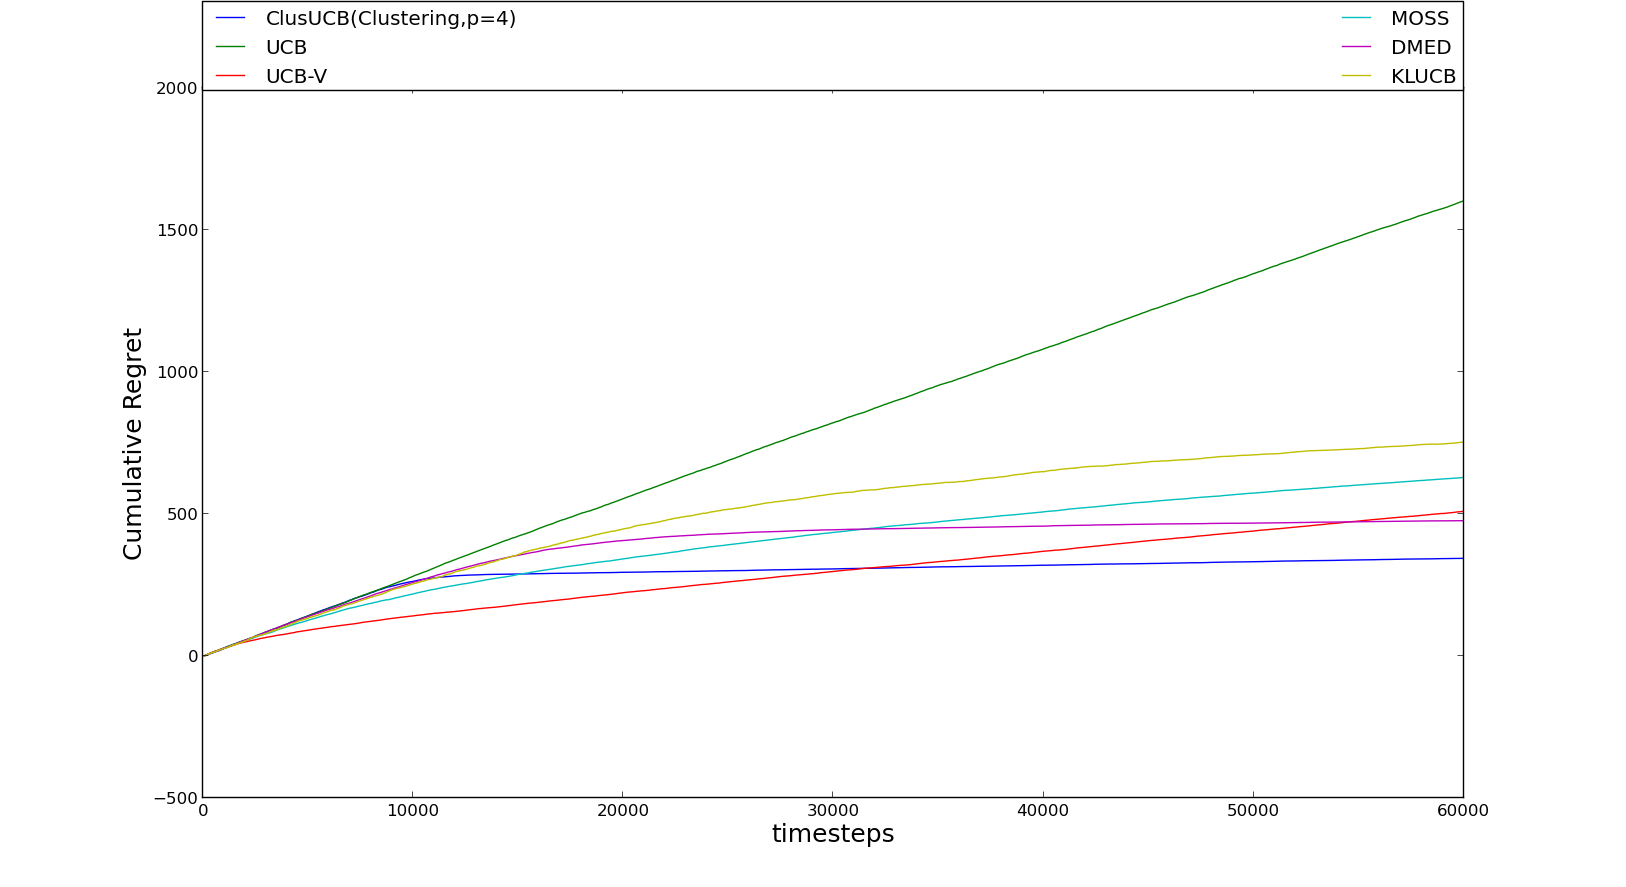
\includegraphics[width=\textwidth]{img/ClusUCB_variousAlgo.png}
%
%\caption{Experiment 1: Regret for various Algorithms. $T=60000$}
%\end{minipage}
%\end{figure}
%
%\hspace{0.1em}
%
%\begin{figure}[!tbp]
%\label{fig:2}
%\begin{minipage}[b]{0.5\textwidth}
%
%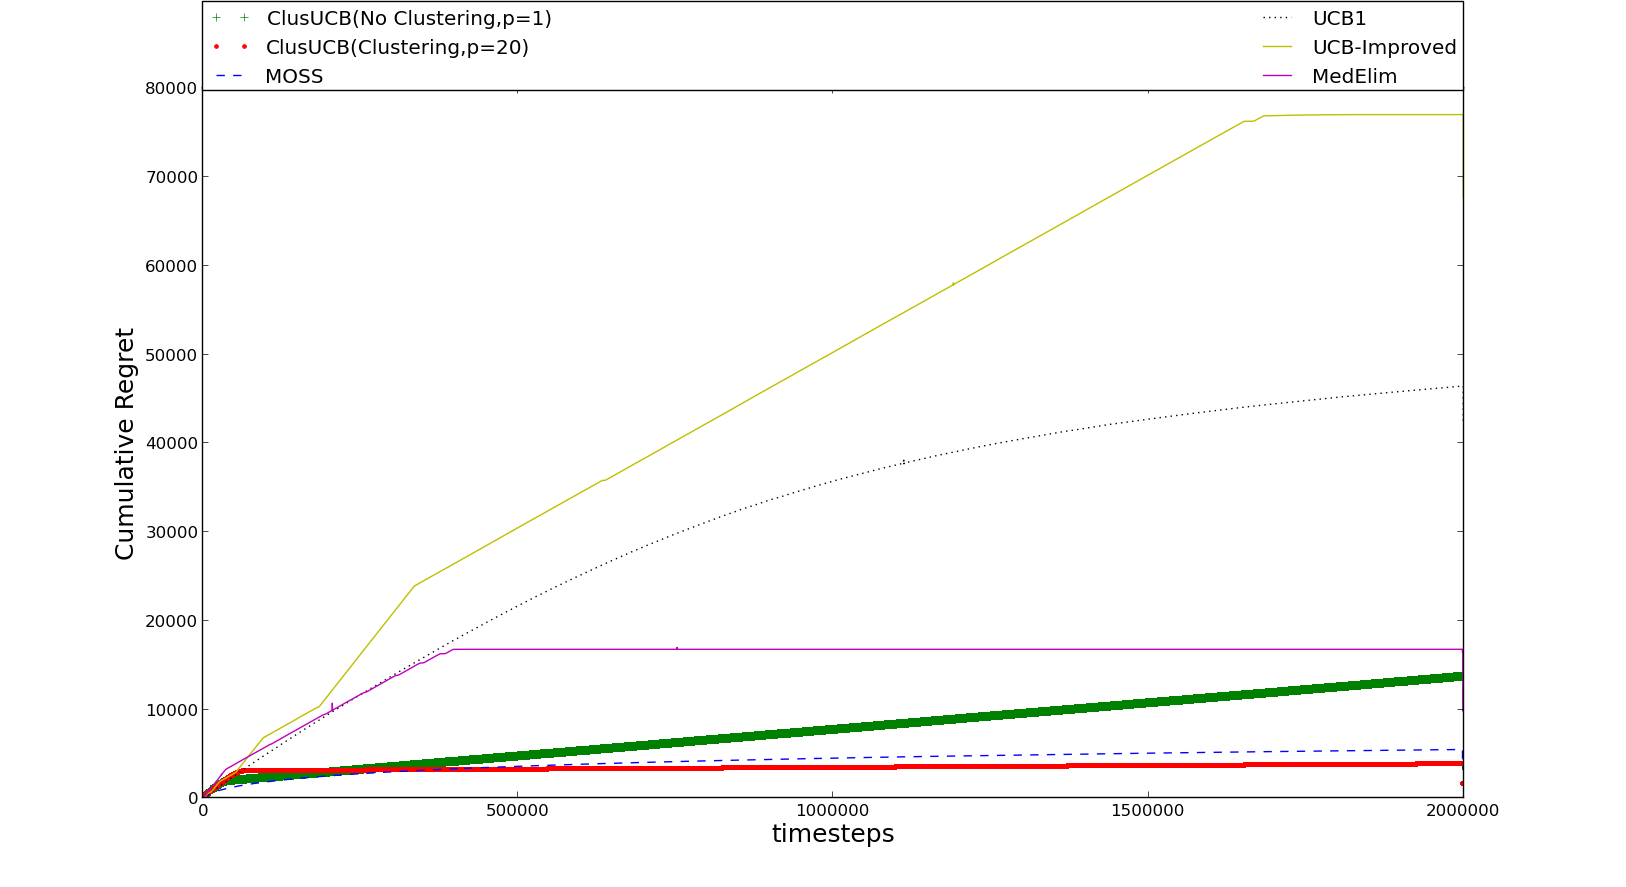
\includegraphics[width=\textwidth]{img/clusUCB_variousAlgo(expt2)_Final.png}
%\caption{Experiment 2: Regret for various Algorithms. $T=2\times 10^{6}$}
%\end{minipage}
%\end{figure}
%
%\hspace{0.1em}
%
%\begin{figure}[!tbp]
%\label{fig:3}
%\begin{minipage}[b]{0.5\textwidth}
%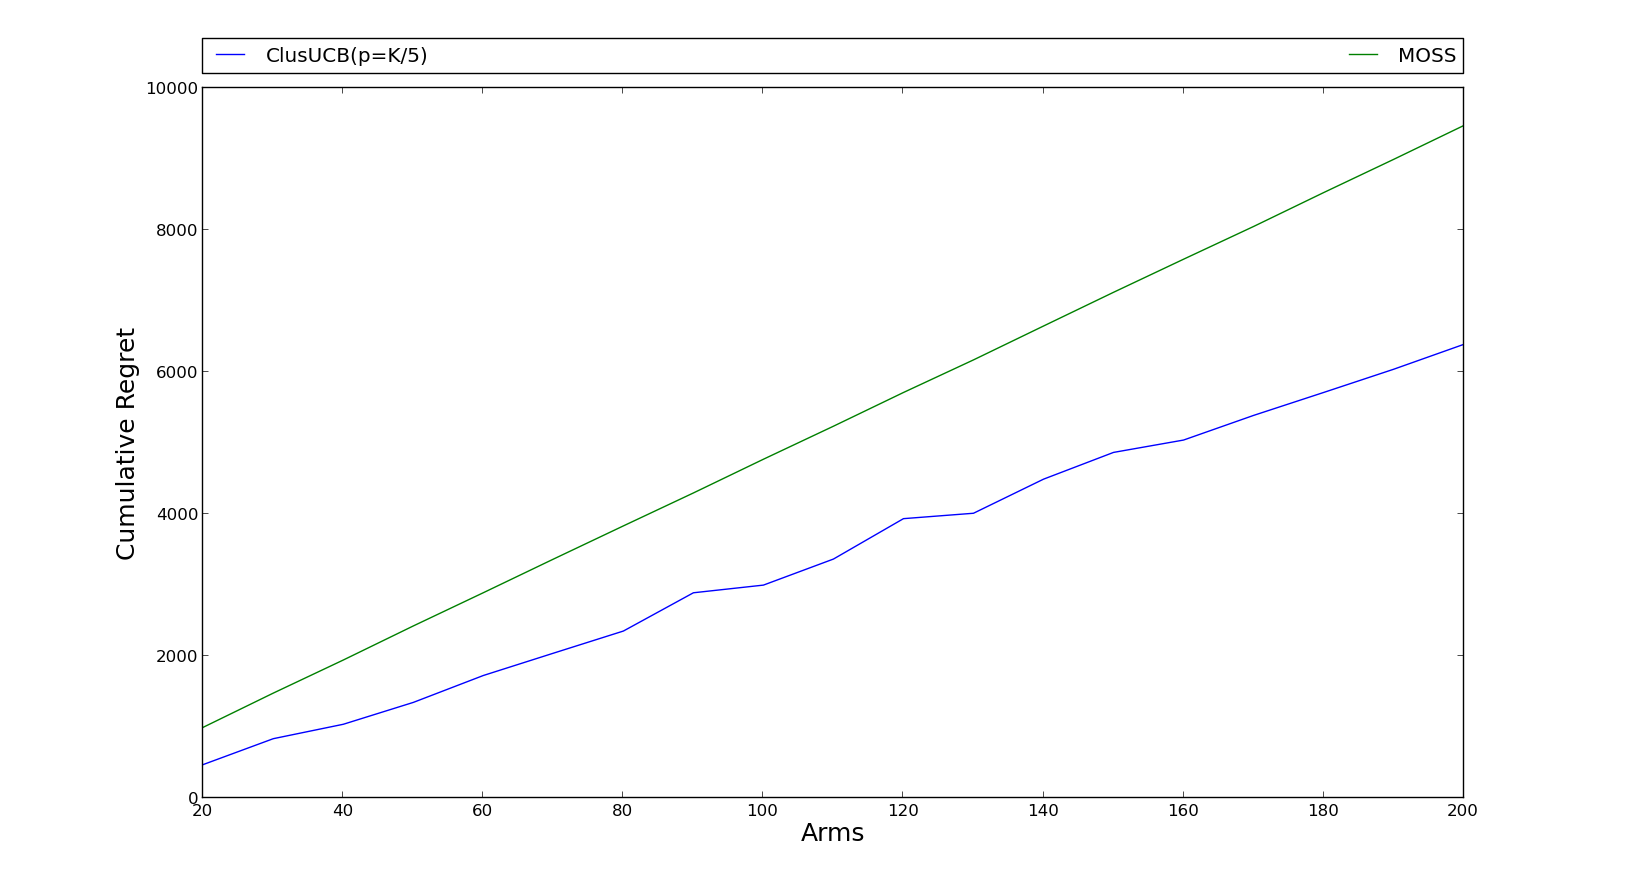
\includegraphics[width=\textwidth]{img/clUCB_MOSS_expt3.png}
%\caption{Experiment 3: Regret Growth for ClusUCB and MOSS . $T=10^{5} + K^{2}\times 10^{4}$ for $K=20$ to $200$}
%\end{minipage}
%\end{figure}
%
%\hspace{0.1em}
%


In the stochastic bandit literature there are several powerful algorithms with and without proven regret bounds. Algorithms like $\epsilon$-greedy(\cite{sutton1998reinforcement}) or softmax(\cite{sutton1998reinforcement}) or UCB-Tuned(\cite{auer2002finite}) has no proven regret bounds. Again algorithms like UCB-$\delta$(\cite{abbasi2011improved}) with proven regret bound better than UCB1  falls within the realm of fixed confidence setting whereas one has to provide the probability of error $\delta$. We also make a distinction between frequentist based approach like the UCB algorithms and the Bayesian approach like the Thompson Sampling(\cite{agrawal2011analysis}). We will not be experimenting against these algorithms but focus on the more recent, algorithms like KL-UCB, DMED, MOSS, UCB1, UCB-V, etc. The codes for KL-UCB and DMED are taken from \cite{CapGarKau12}.

In the experimental setup we use $\psi_{m}=\log T$, $\rho_{s}=\dfrac{1}{2^{2m+1}}$ and $\rho_{a}=\dfrac{1}{2^{4m+1}}$.

The first experiment is conducted over a testbed of $20$ arms for the test-cases involving Bernoulli reward distribution with expected rewards of the arms $r_{i_{a_{i}\neq a^{*}}}=0.07$ and $r^{*}=0.1$. These type of cases are frequently encountered in web-advertising domain. The horizon is set for $T=60000$ and $p=4$ for ClusUCB. The regret is averaged over $100$ independent runs over each timestep and is shown in Figure 1. $6$ algorithms, ClusUCB, MOSS, UCB1, UCB-V, KL-UCB, DMED are run over this testbed and shown in this figure. Here, we see that ClusUCB performs better than all the algorithms mentioned above.

The second experiment is conducted over a testbed of $100$ arms for the test-cases involving Gaussian reward distribution with expected rewards of the arms $r_{i_{a_{i}\neq a^{*}:1-33}}=0.01$, $r_{i_{a_{i}\neq a^{*}:34-99}}=0.06$ and $r^{*}_{i=100}=0.1$. The horizon is set for $T=2\times 10^{6}$ and and $p=20$ for ClusUCB. The regret is averaged over $100$ independent runs over each timestep and is shown in Figure 2. In this test we also show the no-clustering version of ClusUCB algorithm with $p=1$ and keeping all the other parameters same. $4$ other algorithms, MOSS, UCB1, UCB-Improved and Median-Elimination are run over this testbed and shown in this figure. Here, we see that ClusUCB($p=20$) performs better than all the algorithms mentioned above. We also see that no-clustering and using only arm elimination version of algorithm performs worse than the clustering version which stems from the fact that it outputs sub-optimal arm more often than the clustering version.

The third experiment is conducted over a testbed of $20-200$(interval of $10$) arms for the test-cases involving Bernoulli reward distribution with expected rewards of the arms $r_{i_{a_{i}\neq a^{*}}}=0.05$ and $r^{*}=0.1$. The horizon is set for $T=10^{5} + K^{2}\times 10^{4}$ for $K=20$ to $200$ and the parameters of ClusUCB are $p=K/5$ for $K=20$ to $200$. The regret is averaged over $500$ independent runs over each timestep and is shown in Figure 3. We only check the growth of regret for the two algorithms MOSS and ClusUCB over this testbed and see that ClusUCB outperforms MOSS and its growth of regret is lesser than MOSS. The jumps in the graph for ClusUCB happens because of the error(eliminating optimal arm) and the margin of error(in red) is also shown in the graph. 
